\documentclass[11pt]{article}

\usepackage{graphicx}
\usepackage{hyperref}
\usepackage{natbib}

\bibliographystyle{plain}  % or unsrt, alpha, etc.
\setlength{\textwidth}{6.5in}
\setlength{\headheight}{0in}
\setlength{\textheight}{8.0in}
\setlength{\hoffset}{0in}
\setlength{\voffset}{0in}
\setlength{\oddsidemargin}{0in}
\setlength{\evensidemargin}{0in}

\title{LaTex excercise - Problem Set 1}
  
\author{Frederik Holst Knudsen}


\begin{document}

\maketitle

\section{Introduction Paragraph}
I have during my bachelor degree in Copenhagen spent quite a bit of time programming in Python and a tiny bit in ROOT for Pb-Pb collision analysis from the CERN experiment, ALICE. Besides that, I have taken an intermediate Python course during my exchange year at UC Santa Barbara, where I have learned about classes, test oriented programming and more. I have worked with rare-earth ion qubits in Santa Barbara and later on quantum optomechanical membranes in Copenhagen where both projects included a lot of different programming tasks most of which in Python, so I am very excited about the course and to learn more! After my Ph.D. I plan on applying for a Post-Doc and try to pursue a career in academia. 

Best, 
Fred

GitHub: @frederikholst

\label{sec:intro}

\begin{figure}[b!]
\centering
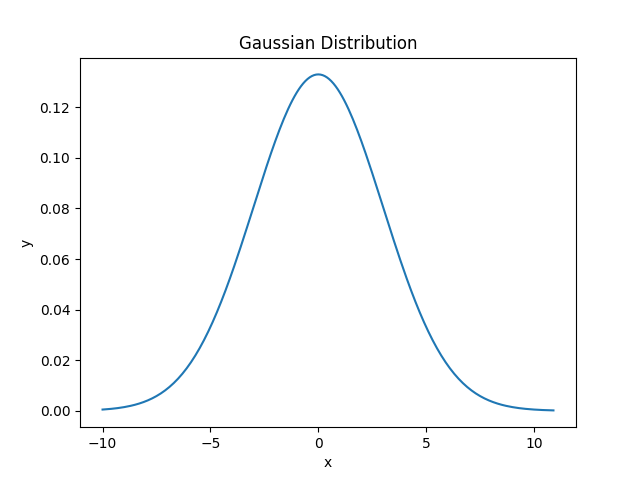
\includegraphics[width=0.5\textwidth]{gaussian.png}
\caption{ \label{fig:example} A normalized Gaussian with sigma=3, and mean=0}
\end{figure}


\end{document}